\vspace{-2mm}
\section{Method}
\label{sec:method}

\textbf{Problem Setup:}
Let $\mathcal{F}$ denote a pre-trained feed-forward multi-view reconstruction model that maps a set of $N$ multi-view images to camera pose and dense geometric predictions. Given a set of input images $\mathcal{I}^R =\{ \mathbf{I}^{\theta_i}_i \}_{i=1}^N$ where each view $\mathbf{I}_i^{\theta_i}$ is captured at an arbitrary in-plane orientation $\theta_i \in [0^\circ, 360^\circ)$. 
Our goal is to recover a scene representation $\hat{\mathcal{G}}$ comparable in quality to that obtained from canonically upright inputs, without retraining or modifying $\mathcal{F}$.

Existing multi-view benchmarks lack systematically rotated images with corresponding ground-truth annotations, making it difficult to evaluate robustness to arbitrary camera orientations.
We therefore develop a Controlled Rotation Synthesis, a procedure that generates rotated multi-view inputs while preserving the underlying scene geometry and avoiding rotation-induced artifacts.
The proposed procedure enables synthetic rotations about all three axes (roll, pitch, and yaw), while avoiding rotation-induced artifacts.
To complement the synthetically rotated benchmarks, we construct RotMV, a real-world benchmark comprising multiple scenes, with each scene containing multi-view images captured at multiple camera orientations for every viewpoint.
% We analyze the performance of ROVER across both types of benchmarks for pointmap reconstruction and camera pose estimation.
In this section, we discuss the controlled rotation synthesis procedure in \cref{sec:rendering_based_rotation} and our proposed method for correcting UprightBias in \cref{sec:ROVER_detail}.

\subsection{Controlled Rotation Synthesis}
\label{sec:rendering_based_rotation}

Our goal is to generate synthetic views by isolating the effect of camera orientation only. 
The created rotation should alter only the camera pose while leaving the scene content and image formation otherwise unchanged.
This is not possible if we naively rotate the images in image space, because it introduces various artifacts like padding, cropping, and resolution changes, as illustrated in \Cref{fig:bicycle_rot}.


Given an upright multi-view sequence $\mathcal I$, we first reconstruct its 3D scene representation $\mathcal G_{\mathrm{3DGS}}$ and corresponding camera poses using a 3D Gaussian Splatting\citep{kerbl3Dgaussians}.
For each view $i$, let its original camera pose be $\mathbf P_i=[\mathbf R_i\mid\mathbf t_i]$, where $\mathbf R_i$ and $\mathbf t_i$ denote the camera rotation and translation, respectively following camera to world convention.
For a synthetic in-plane rotation of $\theta$, represented by $\mathbf R_z(\theta) \in \mathrm{SO}(3)$, the corresponding camera pose is given by $\mathbf P_i^{\theta}=\left[\mathbf R_i\mathbf R_z(\theta)\;\middle|\;\mathbf t_i\right]$.
Analogously, pitch and yaw rotations are synthesized by replacing $\mathbf R_z(\theta)$ with $\mathbf R_x(\theta)$ and $\mathbf R_y(\theta)$, respectively.
The corresponding view is then rendered as:
$$
\tilde{\mathbf I}_i^{\theta_i}=\operatorname{Render}(\mathcal G_{\mathrm{3DGS}},\mathbf P_i^{\theta_i}).$$
The fidelity of $\tilde{\mathbf I}_i^{\theta_i}$ depends on the quality of the reconstructed $\mathcal G_{\mathrm{3DGS}}$, which may vary with the input views and rotation angle $\theta$.
To improve it, we further refine $\mathcal G_{\mathrm{3DGS}}$ using DiFix3D+\citep{wu2025difix3d} Denoiser, and then render the rotated views to obtain the final $\mathbf I_i^{\theta_i}$.
Low-quality renders may still occur and are discarded using a two-stage filtering pipeline \citep{wu2026visualquality}, detailed in the supplementary \cref{sec:image_statistics}. 
Full pipeline details are included in supplementary, specifically the rendering algorithm in \cref{sec:algorithm}, quality filtering procedure and dataset statistics in \cref{sec:image_statistics}.

% \clearpage
\subsection{ROVER}
\label{sec:ROVER_detail}

\begin{wrapfigure}{r}{0.5\textwidth} 
    \vspace{-2em} 
    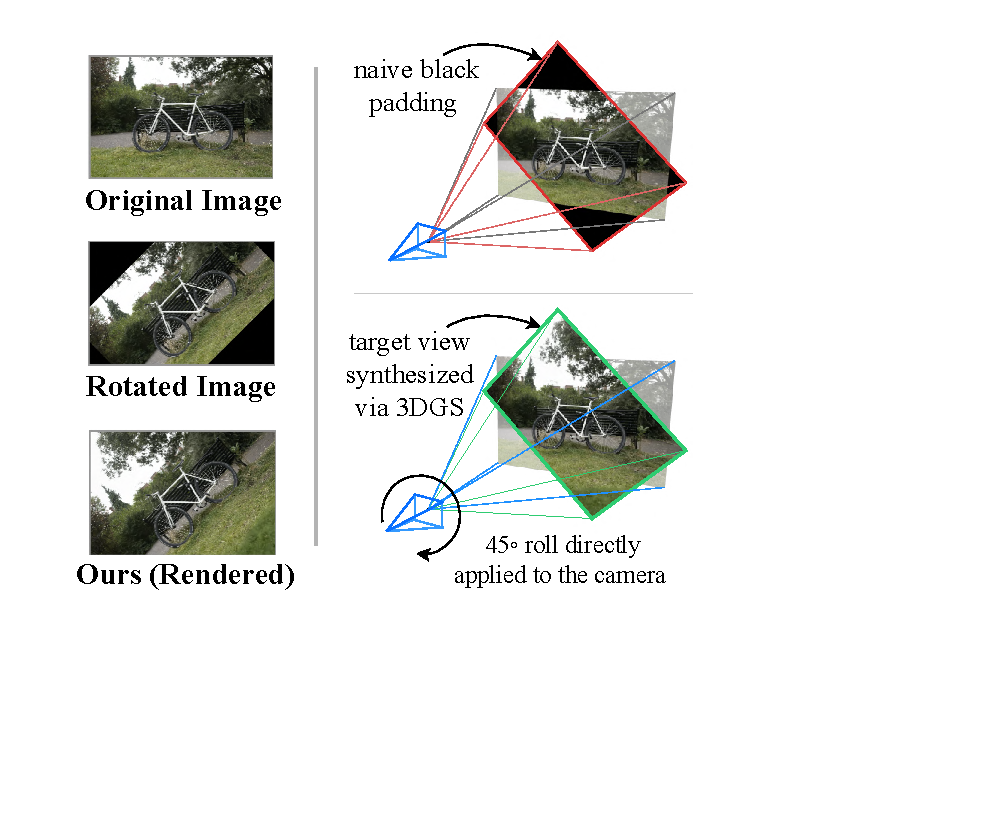
\includegraphics[width=\linewidth]{Figures/fig3/fig3.pdf}
    \caption{\textbf{Controlled Rotation Synthesis.} Naive 2D image rotation (\emph{top right}) introduces black padding, cropping artifacts, or resolution shifts. In contrast, our approach (\emph{bottom right}) applies planar roll $\mathbf{R}_z(\theta)$ directly to the camera pose and synthesizes the target view via 3DGS, generating naturally rotated images.}
    \label{fig:bicycle_rot}
    \vspace{-1em}
\end{wrapfigure}
ROVER constructs a canonicalization operator $T$ that maps an arbitrarily oriented input sequence to the canonical upright orientation expected by the pre-trained reconstruction model.
Our method realizes the canonicalization operator $T$ by decomposing it into two sequential operators, $T=C\circ E$, where $E:\mathcal{I}^R\rightarrow\hat{\Theta}$ estimates the canonical orientation of each image in the input sequence, with $\hat{\Theta}=\{\hat{\theta}_i\}_{i=1}^{N}$ denoting the estimated orientations, and $C:(\mathcal{I},\hat{\Theta})\rightarrow\mathcal{I}^{\mathrm{can}}$ applies the corresponding transformations to produce the canonicalized image sequence. 
Since both operators act entirely in image space, ROVER requires neither retraining nor architectural modifications to the underlying feed-forward reconstruction model.

% \textbf{Estimating the Canonical Orientation:}

% The orientation estimation operator $E$ determines the canonical 
% orientation of each image in the input sequence. To implement $E$, 
% we require a representation whose feature geometry varies 
% predictably with image orientation. We use a frozen DINOv2 
% encoder $\phi$ \citep{oquab2023dinov2}, motivated by an empirical 
% observation established in the supplementary: patch-level embeddings 
% from DINOv2 exhibit maximal spatial variance when the input image 
% is presented in its canonical upright orientation. We attribute 
% this to the KoLeo regularizer \citep{sablayrolles2018spreadingkoleoregularizer} 
% used during DINOv2 training, which explicitly encourages uniform 
% dispersion of patch embeddings, thereby inducing an 
% orientation-sensitive structure in the representation space.

% For each input image $\mathbf{I}$ and candidate orientation $\theta \in \Theta$, we obtain patch embeddings $\mathbf{Z}_{\theta} = \phi(\mathbf{I}^{\theta}) = \{\mathbf{z}_j^\theta\}_{j=1}^M$, $\mathbf{z}_j^\theta \in \mathbb{R}^D$, and estimate the canonical orientation as:
% %
% \begin{equation}
% V(\theta) = \frac{1}{M}\sum_{j=1}^{M}
% \left\|\mathbf{z}_j^\theta - \bar{\mathbf{z}}^\theta\right\|_2^2,
% \qquad
% E(\mathbf{I}) = \arg\max_{\theta \in \Theta}\, V(\theta),
% \end{equation}
% where $\bar{\mathbf{z}}^\theta = \frac{1}{M}\sum_{j=1}^{M} 
% \mathbf{z}_j^\theta$.

% To achieve $1^\circ$ resolution while avoiding exhaustive 
% evaluation over all $360$ candidates, we employ a 
% coarse-to-fine search. We first evaluate $V(\theta)$ over 
% a coarse grid $\Theta_\text{coarse} = \{15^\circ \times k 
% \mid k = 1, \ldots, 24\}$, obtaining a coarse estimate 
% $\theta_c = \arg\max_{\theta \in \Theta_\text{coarse}} V(\theta)$. 
% We then refine within $[\theta_c - 7^\circ, \theta_c + 7^\circ]$ 
% at $1^\circ$ intervals. 

% \textbf{Applying the Canonicalization Operator:}
% Given the estimated orientation $\hat{\theta}=E(\mathbf{I})$, the canonicalization operator $C$ restores the input image to its canonical orientation by rotating it using the estimated correction angle.
% Formally, the canonicalized image is obtained as $\mathbf{I}^{\mathrm{can}}\approx\mathrm{R}_z(\mathbf{I},\hat{\theta})$, where the approximation reflects that $\hat{\theta}$ is estimated with finite angular resolution.
% Applying $C$ independently to every image in the input sequence produces the canonicalized image sequence $\mathcal{I}^{\mathrm{can}}=\{\mathbf{I}_i^{\mathrm{can}}\}_{i=1}^{N}$, which is then provided directly to the original feed-forward reconstruction model for scene reconstruction without retraining or modifying its architecture.


% Given the estimated orientation $\hat{\theta} = E(\mathbf{I})$, 
% the canonicalization operator $C$ restores the image to its 
% canonical upright orientation by applying a corrective in-plane 
% rotation $ \mathbf{I}^{\mathrm{can}} = C(\mathbf{I}) = \mathbf{I}^{-\hat{\theta}}$ where $\mathbf{I}^{-\hat{\theta}}$ denotes the image rotated 
% by $-\hat{\theta}$, correcting for the estimated deviation 
% from the canonical orientation. Applying $C$ independently 
% to every image in the input sequence yields the canonicalized 
% sequence $\mathcal{I}^{\mathrm{can}} = 
% \{\mathbf{I}_i^{\mathrm{can}}\}_{i=1}^{N}$, which is passed 
% directly to $\mathcal{F}$ for scene reconstruction without 
% any retraining or architectural modification.

% \AD{@Badri Please re-write this section. What is that key insight which led us to go with the variance based method. 1.) Produce some $V(\theta)$ plots for different rotations. 2.) Also, describe the method using algorithm. 3.) Fix the notations for rotation, upright set, rotated set, candidate angles etc. thorughout the manuscript. Best way to structure this section: Observation, Score computation, Method, RUn-time analysis. }

% We observe that (validated in the supplementary): the final layer patch-level embeddings of a 
% frozen DINOv2 encoder $\phi$ \citep{oquab2023dinov2} exhibit 
% maximal spatial variance when the input image is presented in its canonical upright orientation, and this variance is lower as the image deviates from upright. We attribute this to the KoLeo regularizer \citep{sablayrolles2018spreadingkoleoregularizer} used during DINOv2 training, which explicitly encourages uniform dispersion of patch embeddings. Since natural upright images dominate the pretraining distribution, the encoder implicitly learns representations that are most dispersed for canonical orientations, making patch embedding variance a reliable proxy for image uprightness. Variance plots across datasets and scenes, confirming that DINOv2 patch embedding variance peaks at the canonical upright orientation, are provided in supplementary \cref{sec:ROVER_empirical_plots}.
\textbf{Estimating the Canonical Orientation:}
We made an important observation that enabled us to estimate orientation directly from the representations of DINOv2 encoder.
DINOv2 employs the KoLeo regularizer \citep{sablayrolles2018spreadingkoleoregularizer}, which encourages uniform dispersion of the learned embeddings.
This provides a natural basis for measuring the spatial variance of its patch-level embeddings.
Since the DINOv2 pretraining distribution is dominated by naturally upright images, we hypothesize that this dispersion is strongest when an image is presented in its canonical upright orientation.
We observe that the spatial variance of final-layer patch embeddings indeed peaks at the canonical upright orientation and decreases as the image deviates from upright, consistently across datasets and scenes (provided in supplementary \cref{sec:ROVER_empirical_plots}).
This makes patch embedding variance a reliable proxy for image uprightness, allowing us to estimate the canonical orientation by maximizing the variance over candidate orientations.
For each input image $\mathbf{I}$ and candidate orientation $\theta \in \Theta$, we compute the DINOv2 patch embeddings $\mathbf{Z}^{\theta}=\phi(\mathbf{I}^{\theta})=\{\mathbf{z}_j^\theta\}_{j=1}^{M}$ with mean embedding $\bar{\mathbf{z}}^\theta$, and estimate the canonical orientation $\hat{\theta}$ by maximizing their spatial variance:
\begin{equation*}
V(\theta) = \frac{1}{M}\sum_{j=1}^{M}
\left\|\mathbf{z}_j^\theta - \bar{\mathbf{z}}^\theta\right\|_2^2
\quad\Longrightarrow\quad
E(\mathbf{I}) = \hat{\theta} = \arg\max_{\theta \in \Theta} V(\theta).
\end{equation*}
\vspace{-2mm}

% For each input image $\mathbf{I}$ and candidate orientation 
% $\theta \in \Theta$, we rotate the image by $\theta$ and pass 
% it through the frozen DINOv2 encoder to obtain patch embeddings 
% $\mathbf{Z}_{\theta} = \phi(\mathbf{I}^{\theta}) = 
% \{\mathbf{z}_j^\theta\}_{j=1}^M$. 
% The orientation score $V(\theta)$ is defined as 
% the spatial variance of these embeddings:
% \begin{equation}
% V(\theta) = \frac{1}{M}\sum_{j=1}^{M}
% \left\|\mathbf{z}_j^\theta - \bar{\mathbf{z}}^\theta\right\|_2^2,
% \qquad
% E(\mathbf{I}) = \hat{\theta} = \arg\max_{\theta \in \Theta}\, V(\theta).
% \end{equation}
% where $\bar{\mathbf{z}}^\theta = \frac{1}{M}\sum_{j=1}^{M}\mathbf{z}_j^\theta$ and the orientation estimation operator $E$ selects the candidate 
% orientation that maximizes the variance score.

\textbf{Applying the Canonicalization Operator:}
Given $\hat{\theta}$, the canonicalization operator $C$ applies a corrective rotation to restore the image to its upright orientation $\mathbf{I}^{\mathrm{can}} = C(\mathbf{I}) = \mathbf{I}^{-\hat{\theta}}$. Applying $T = C \circ E$ independently to every image in $\mathcal{I}^R$ yields the canonicalized sequence $\mathcal{I}^{\mathrm{can}} = \{\mathbf{I}_i^{\mathrm{can}}\}_{i=1}^{N}$, which is passed to feed-forward model $\mathcal{F}$.
Exhaustive evaluation of $V(\theta)$ over all $360$ integer-degree candidates requires $360$ DINOv2 forward passes per image. 
We instead employ a coarse-to-fine search that requires only two batched DINOv2 forward passes per multi-view sequence at inference time. 
In the coarse stage, we evaluate $V(\theta)$ over $\Theta_\text{coarse} = \{15^\circ \times k \mid k = 1, \ldots, 24\}$ and obtain $\theta_c = \arg\max_{\theta \in \Theta_\text{coarse}} V(\theta)$.
In the fine stage, we evaluate $V(\theta)$ within $[\theta_c - 7^\circ,\, \theta_c + 7^\circ]$ at $1^\circ$ intervals.
Since all candidate rotations for a stage can be batched, each stage requires only a one DINOv2 forward pass for the entire multi-view sequence. We include results for latency in \cref{sec:additional_results_suppl} and a full algorithmic description is provided in the supplementary \cref{alg:var_alg}.


% Exhaustive evaluation of $V(\theta)$ over all $360$ integer-degree candidates requires $360$ DINOv2 forward passes per image. We instead employ a coarse-to-fine search strategy. In the coarse stage, we evaluate $V(\theta)$ over $\Theta_\text{coarse} = \{15^\circ \times k \mid k = 1, \ldots, 24\}$, obtaining $\theta_c = \arg\max_{\theta \in \Theta_\text{coarse}} V(\theta)$. In the fine stage, we refine within $[\theta_c - 7^\circ,\, \theta_c + 7^\circ]$ at $1^\circ$ intervals. Since both stages evaluate a small, fixed set of candidate rotations, we batch every image together with its candidate-rotation variants and evaluate each stage in a single forward pass, thus ROVER requires only two batched DINOv2 forward passes in total for an entire multi-view sequence, one for the coarse stage and one for the fine stage. A full algorithmic 
% description is provided in the supplementary 
% (\cref{alg:var_alg}). Because ROVER operates purely as an image-space preprocessing step using its own frozen DINOv2 encoder, it requires no modification to $\mathcal{F}$'s architecture and adds no additional parameters, making it plug-and-play: the same procedure can be prepended to any feed-forward reconstruction model. Our method uses an off-the-shelf, frozen DINOv2 encoder for orientation estimation and therefore requires no additional trained parameters; the coarse-to-fine search adds only two batched DINOv2 forward passes in total per multi-view sequence at inference time, independent of the downstream reconstruction model $\mathcal{F}$.

